%  Robotics Text  by Jacob Rosen and Blake Hannaford
% (c) 2007  Jacob Rosen and Blake Hannaford
%

\chapter{Teleoperation}

\section{Problem Statement and Learning Objectives}
% Problem Statement and Learning Objectives for Chapter 14



%%%%%%%%%%%%%%%%%%%%%%%%%%%%%%%%%%%%%%%%%%%%%%%%%%%%%%%%%%%%%%%%%%%%%%%%%%%%%%%%%%%%%%%%%%%%%%
%
%
%                Combined Systems and Networks
%
%


%\begin{slide}

\section*{Kinematics of Teleoperation Systems}

%%%%** Section 1
\section{Introduction}
This chapter will introduce analytical models of teleoperation systems with multiple degrees of freedom.

We will focus on how to convert motion and force information as it flows back 
and forth in a remotely controlled telemanipulation system.

Students completing this chapter will be able to
\begin{itemize}
\item Explain and diagram at the block diagram level historical and current standard
remote control schemes for teleoperation, including methods with force feedback to the 
human operator. 
\item Define and formulate design requrements for scaling and indexing (offsetting)
between the human operator's motion and the remote manipulator's motion. 
\item Analyze the relevant coordinate frames for teleoperation with indexing. 
\item Apply dynamical systems concepts to electromechanical networks to study 
flows of energy, force, and motion in teleoperation systems.
\item Model teleoperation systems with force feedback in terms of 2-port networks. 
\end{itemize}


\section{Special Historical Note}
Going back to it's founding in the 1940's, the teleoperation field used language
which is fundamentally offensive to many groups (especially Black-Indiginous-and People
of Color (BOPIC) people).  Specifically, the side of the system interfacing the 
human operator was referred to as "master" and the remote robot side the "slaves" side. 

This book adopts the terms "Leader" and "Follower" to denote the human-facing and 
task/environment-facing sides of the teleoperation system. 


	%<*>
%\end{slide}
%\begin{slide}
%%%%** Section 2
\section{Four Approaches}
\begin{enumerate}
	\item Joint Rate Control
	\item Resolved Rate Control
	\item Leader-Follower Control
	\item Generalized Leader-Follower Control
\end{enumerate}


%%%%** Section 2.1
\subsection{Joint Rate Control}

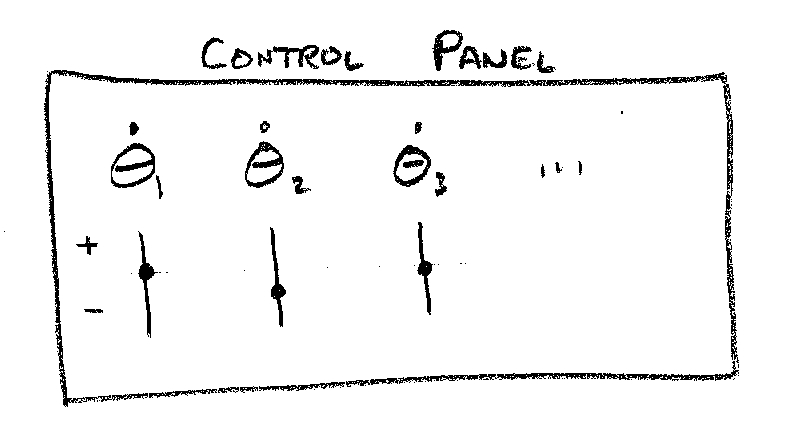
\includegraphics[width=4.0in]{figs14/00398.jpg}

A basic control panel with knobs to control the rate of each joint.

Examples:   Hydraulic construction Equipment

Must have spring return to zero!

\subsubsection*{Advantage}
Cheap!
\subsubsection*{Disadvantage}
Human must do inverse kinematics in their heads.


	%<*>
%\end{slide}
%\begin{slide}

%%%%** Section 2.2
\subsection{Resolved Rate Control}

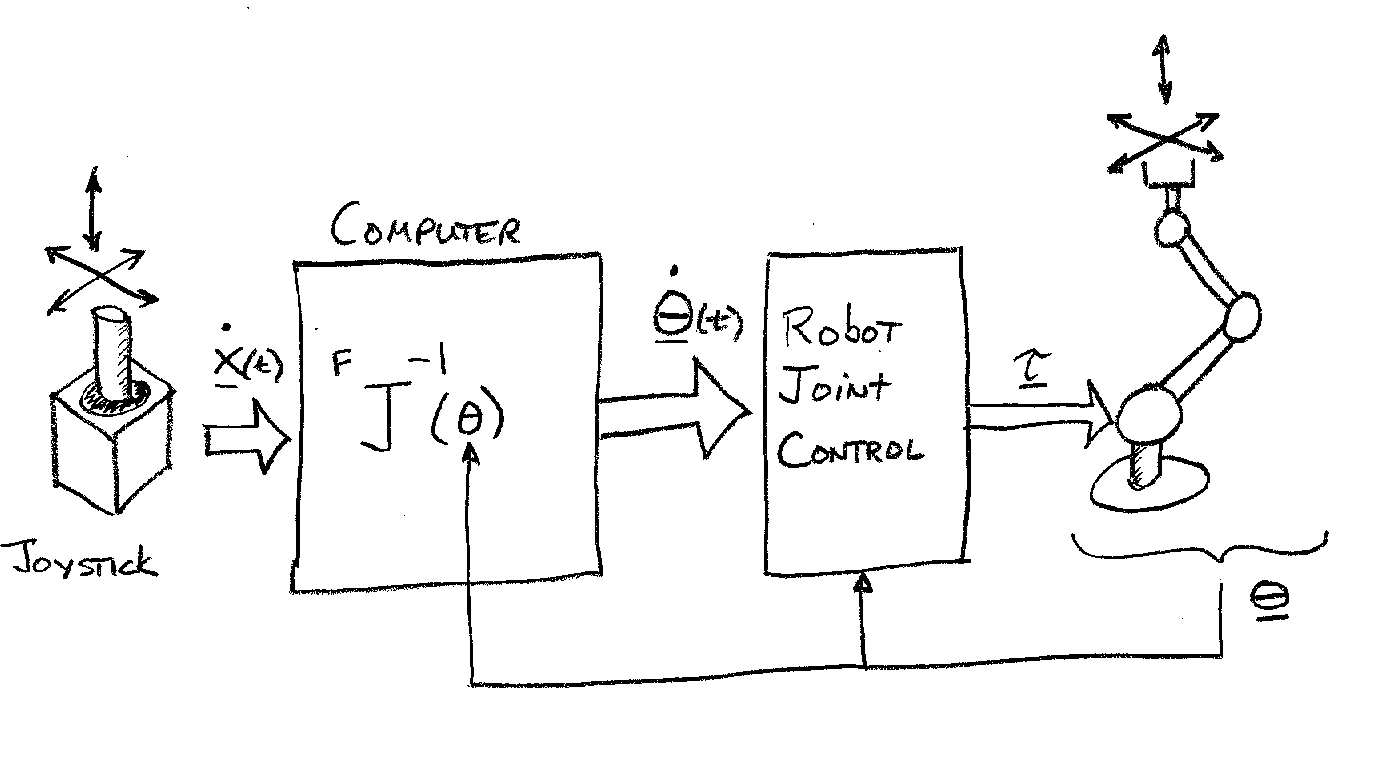
\includegraphics[width=4.0in]{figs14/00399.jpg}


\subsubsection*{Advantages}
\begin{itemize}
	\item Modest computational requirements
	\item Can be adapted to task (i.e. change of reference frame or reference point).

	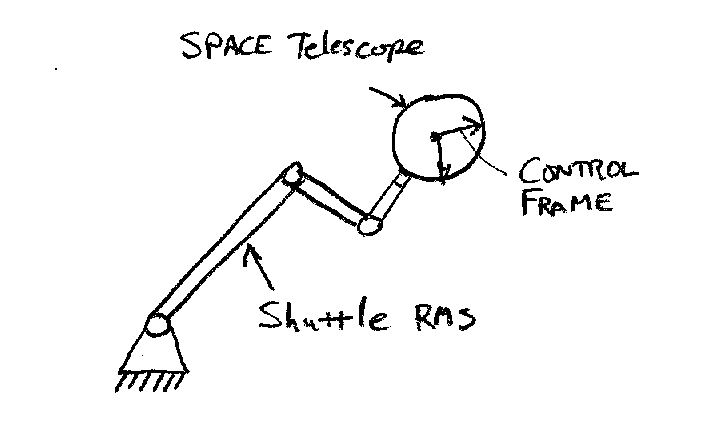
\includegraphics[width=4.0in]{figs14/00400.jpg} 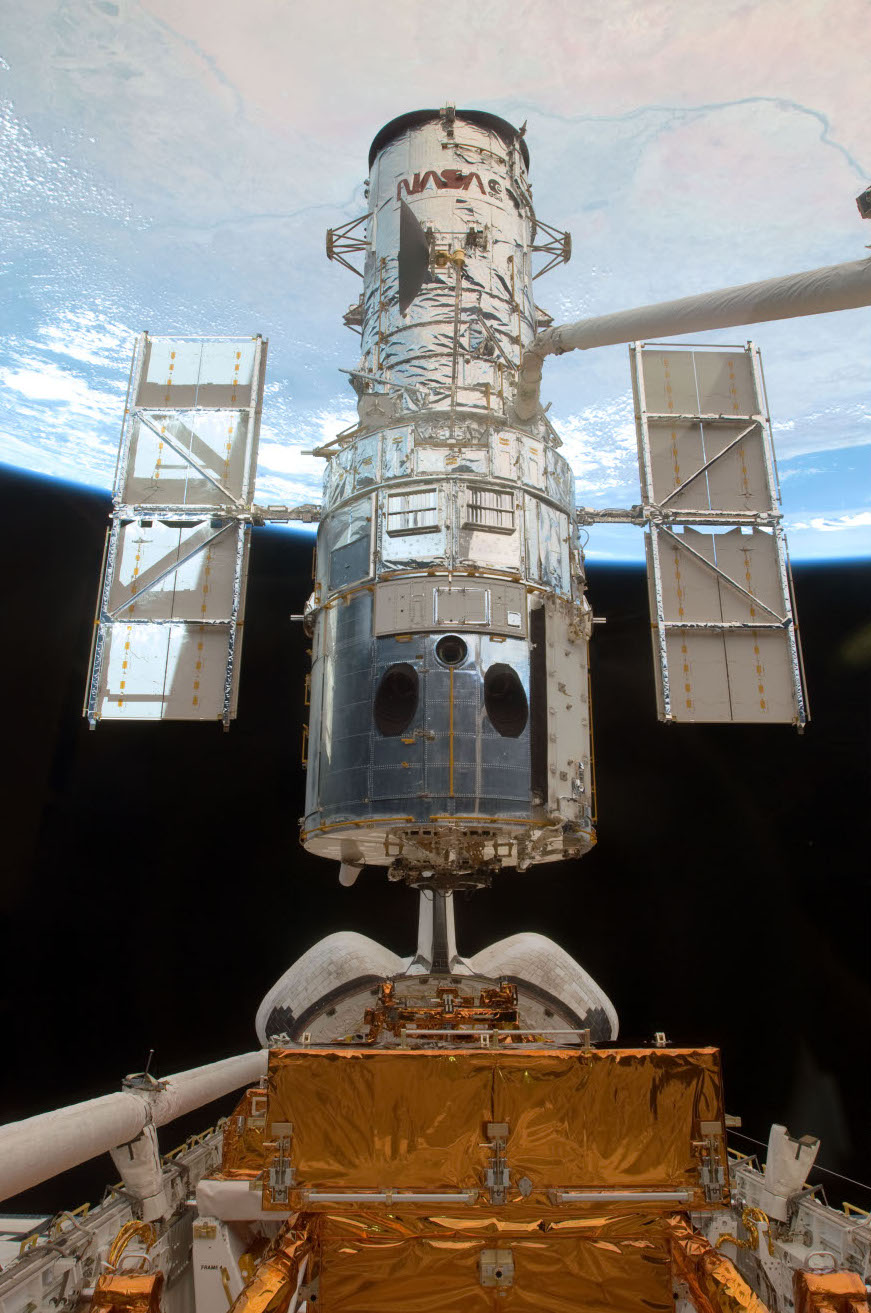
\includegraphics[width=2.5in]{figs14/hubbleRMS.eps}	%<hn>

        Example of the Hubble space telescope manipulated by space shuttle robot arm (RMS).   The reference frame for resolved rate control can be programmed to the center of mass of the telescope or any convenient point. 	%<hn>
\end{itemize}

 

\subsubsection*{Disadvantages}
\begin{itemize}
   \item Cognitive Load
           \begin{itemize}
                 \item Operator must differentiate desired trajectory.
		 \item Rate control of orientation is difficult
            \end{itemize}
   \item Need to watch out for singualrities in Jacobian Matrices.

System may demand infinite joint rates from follower robot.
\end{itemize}


	%<*>



%\end{slide}
%\begin{slide}

%%%%** Section 2.3
\subsection{Leader Follower Control}

This situation describes teleoperators where the leader and follower devices are kinematically the same.

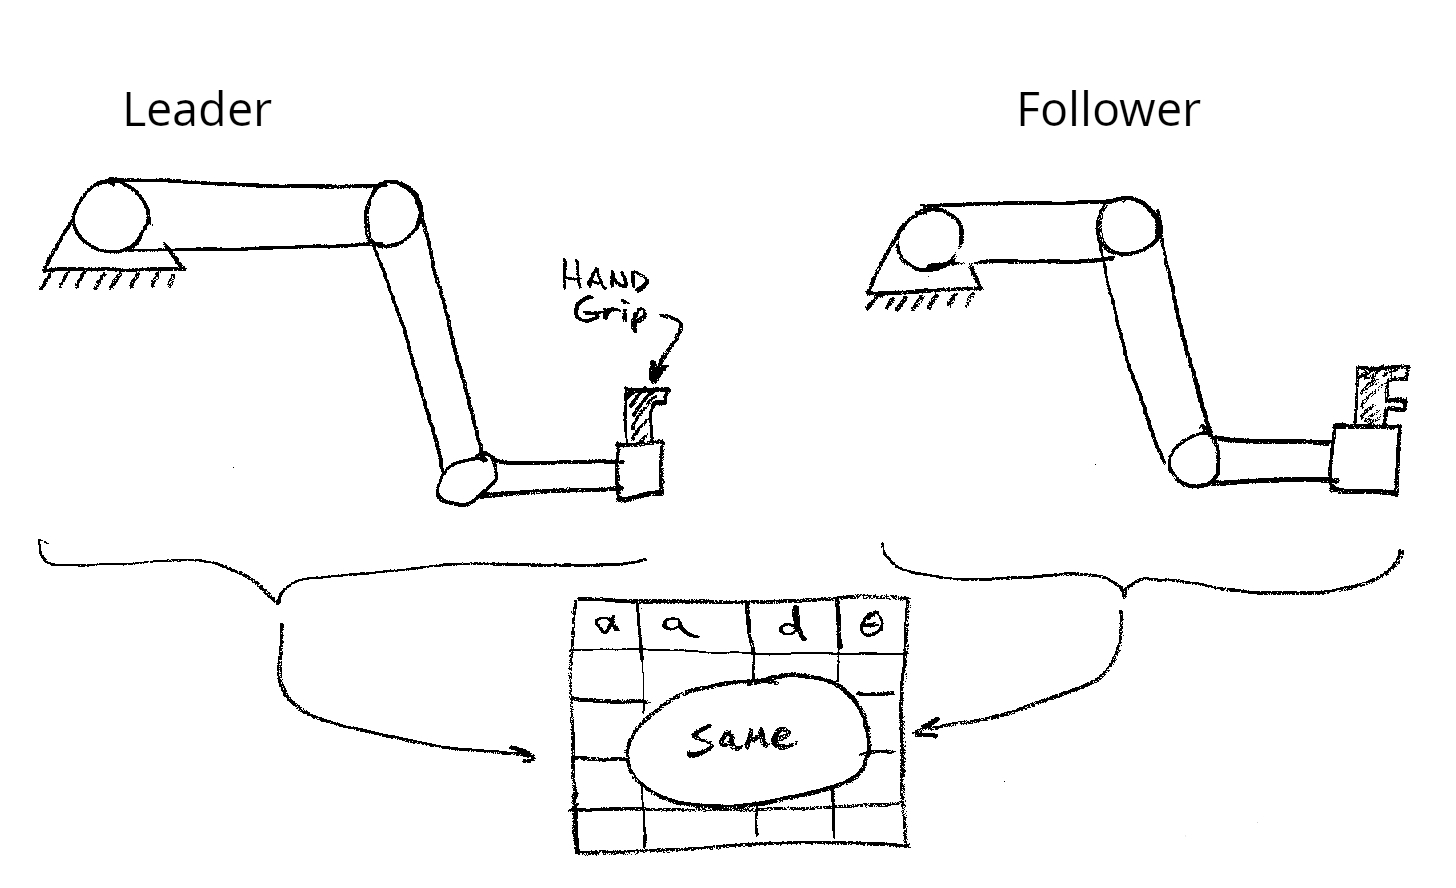
\includegraphics[width=4.0in]{figs14/00401.jpg}

Controller must make sure that
\bq
\theta_F = \theta_L
\eq
Since the kinematic parameters (i.e. Denavit Hartenberg Parameters) are the same, this implies
\bq
^0_6T_F = ^0_6T_L
\eq
Also, if
\[
\tau_L = \tau_F
\]
then
\bq
F_L = F_F
\eq

One such controller is

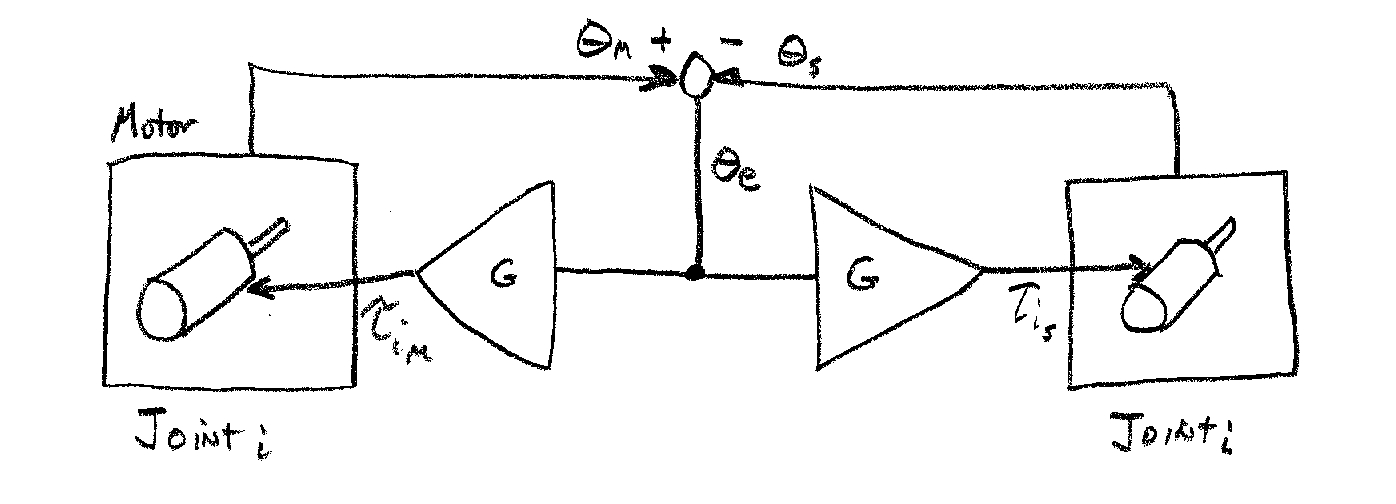
\includegraphics[width=4.0in]{figs14/00403.jpg}

%\end{slide}
%\begin{slide}


\subsubsection*{Advantages}
\begin{itemize}
   \item Simple Architecture (e.g. six separate analog controllers in 1950's).
   \item Good operator interface (1:1 motion and force feedback)
\end{itemize}

\subsubsection*{Disadvantages}
\begin{itemize}
   \item Leader and Follower must be same design.
   \item Leader and Follower must be in same configuration
   \item Can't index or scale the motion.
\end{itemize}

%\end{slide}
%\begin{slide}

%%%%** Section 2.4
\subsection{Indexing and Scaling}
%%%%** Section 2.4.1
\subsubsection{Definitions}

\begin{description}
\item [Indexing:] Provision of an arbitrary offsett between leader and follower configurations.
\item [Scaling:]  Ability to multiply position commands by an arbitrary constant.
\end{description}


%%%%** Section 2.4.2
\subsubsection{Problems with Scaling and Indexing}
Consider a Leader/follower system which is moved by $\Delta x_i$ at the leader resulting in follower motion $\Delta x_0$.

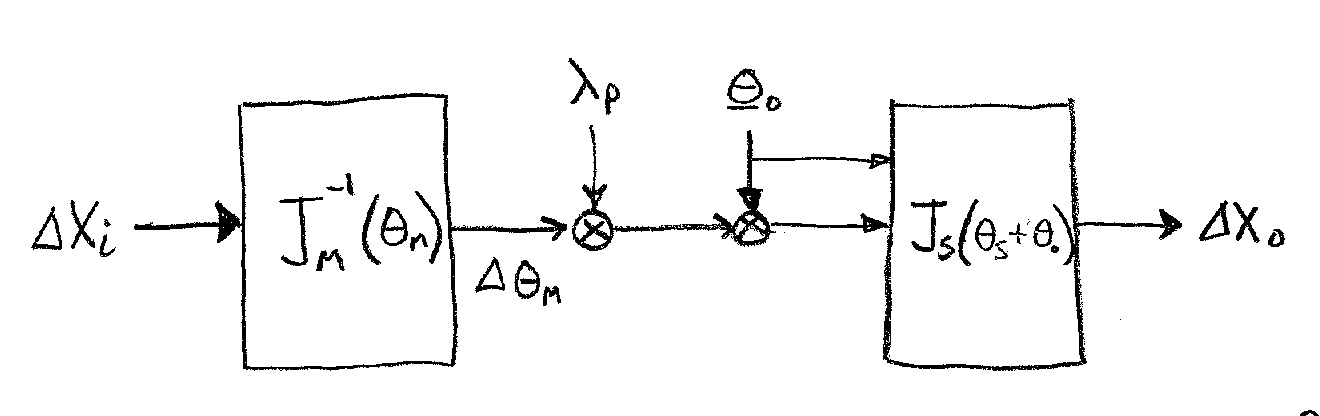
\includegraphics[width=4.0in]{figs14/00402.jpg}


if $\lambda_p =1$ and $\theta_0 = 0$, then
\bq
\theta_L = \theta_F, J_L(\theta_L) = J_F(\theta_F)
\eq
	%<*>

and

\[
\Delta x_0 = J_F(\theta_F)J^{-1}_L(\theta_L)\Delta x_i
\]
\[
\Delta x_0 = \Delta x_i
\]

%\end{slide}
%\begin{slide}

Consider indexing:

if $\theta_0 \ne 0$
\[
\theta_F = \theta_L + \theta_0
\]
\[
J_F(\theta_L+\theta_0)J^{-1}_L(\theta_L) \ne I
\]

%\end{slide}
%\begin{slide}

Consider scaling:

if $\lambda_p \ne 1$
\[
\theta+s = \lambda_p\theta_L
\]
\[
J_F(\lambda_p\theta_L)J^{-1}_L(\theta_L) \ne \lambda_p I
\]



%\end{slide}
%\begin{slide}

%%%%** Section 2.5
\subsection{Generalized Leader Follower Control}

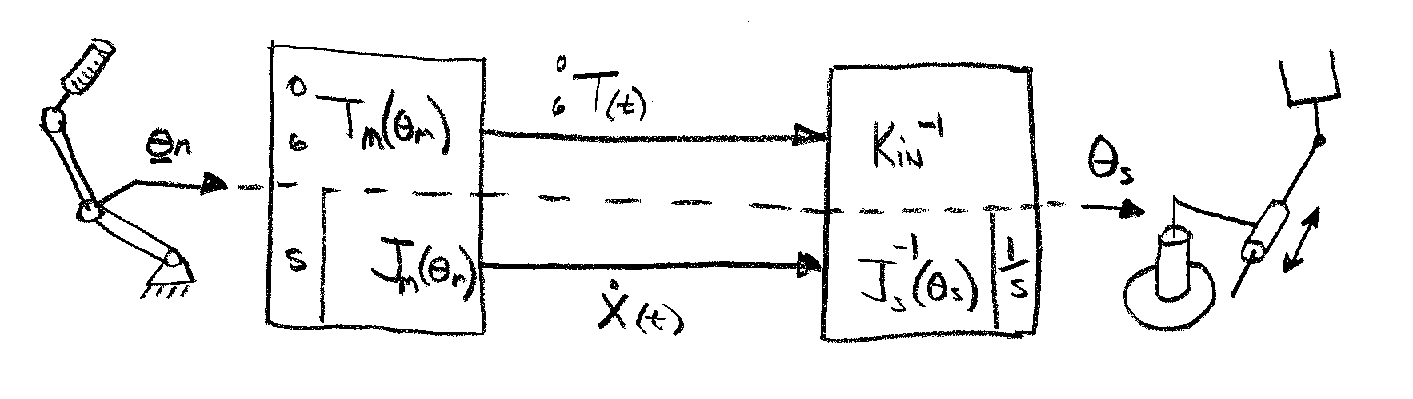
\includegraphics[width=4.0in]{figs14/00404.jpg}

Leader and Follower mechanisms kinematically different.

Communication options:

1) send 4x4 matrices indicating end effector frame (absolute coordinates)

2) send cartesian increment commands.

%\end{slide}
%\begin{slide}

%%%%** Section 2.5.1
\subsubsection{Indexing (using 4x4 Frames)}

1) No indexing:

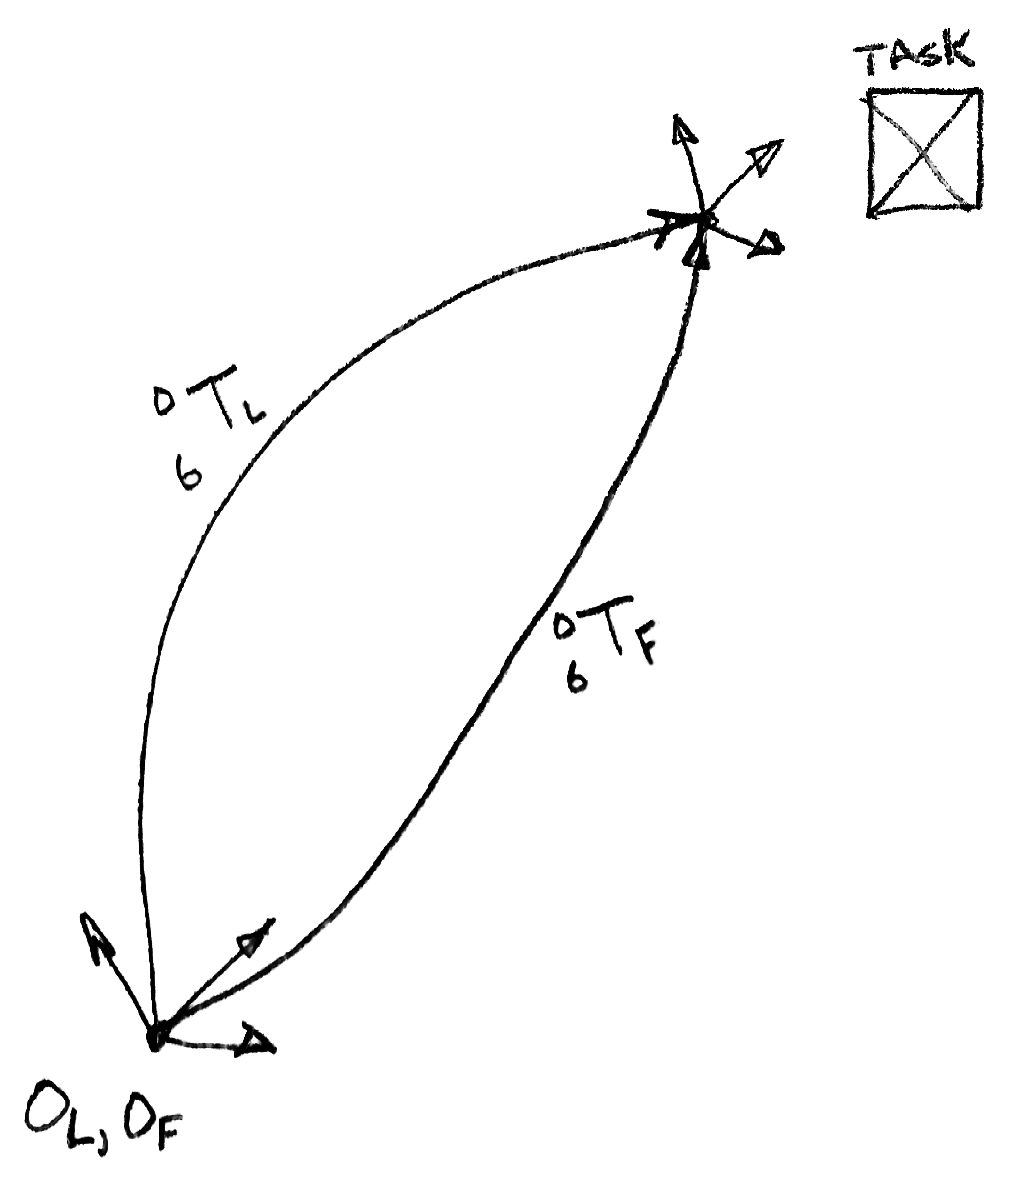
\includegraphics[width=3.0in]{figs14/00405a.png}

 The leader and follower frames are superimposed on the same points(!)    There is actually of course an offset between the frames but mathematically we ignore it to lock their motions together. 	%<hn>


%\end{slide}
%\begin{slide}

2) With an index offset:

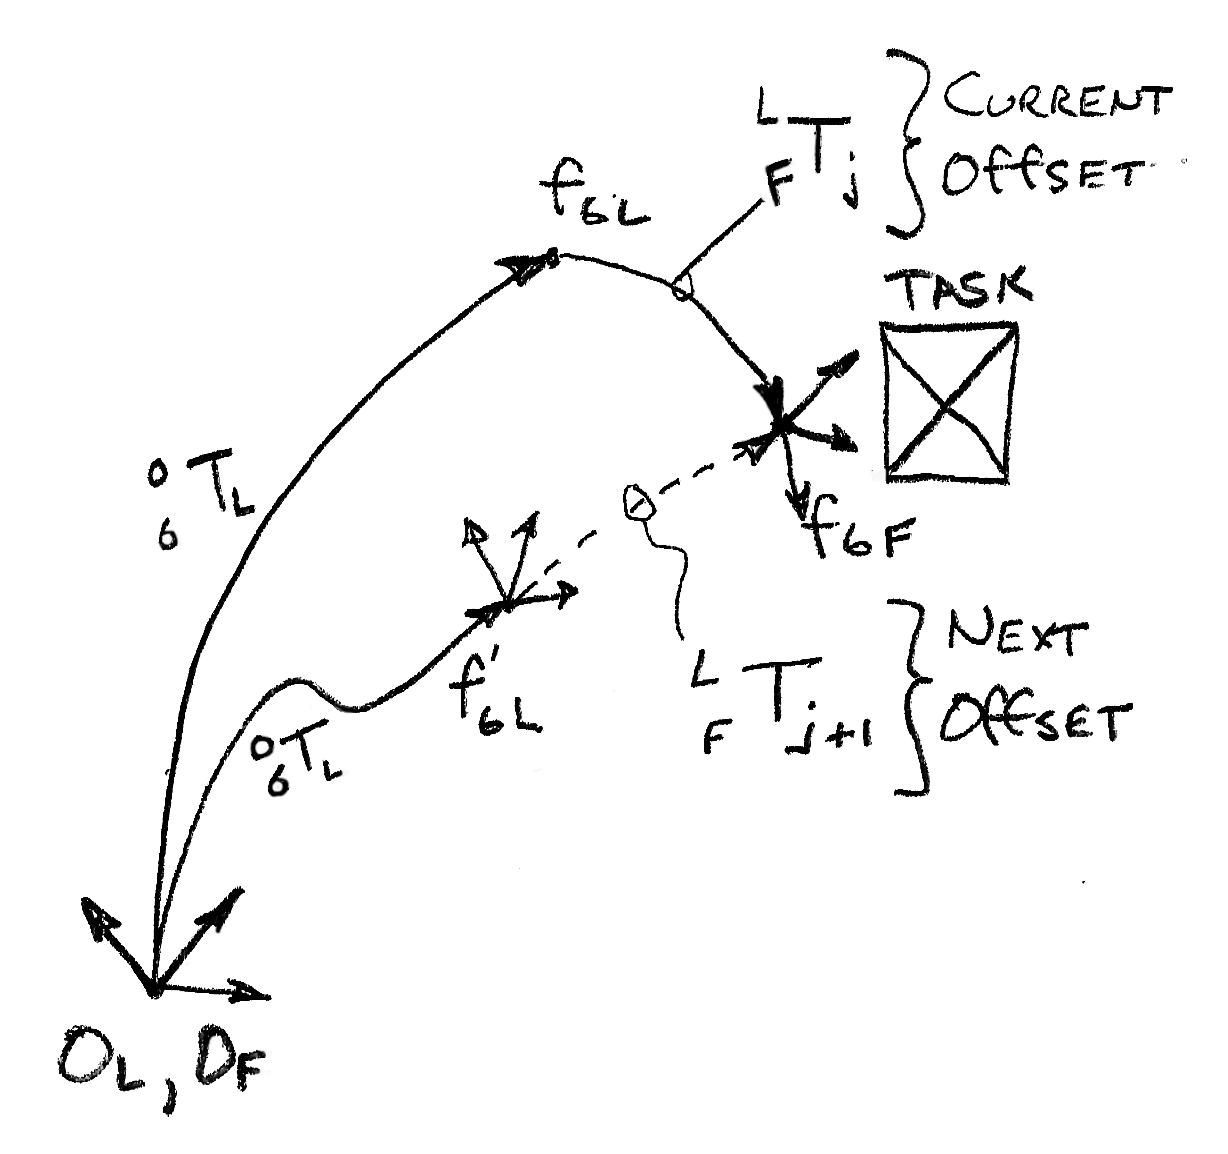
\includegraphics[width=3.0in]{figs14/00406a.png}

 Operator first works with index offset $j$, and then creates a new offset $^L_FT_{j+1}$ by pressing a button and moving the leader to a new location (with the follower frozen).  Analyzing the diagram, 	%<hn>

\bq
^L_FT_{j+1} = \left ( ^6_0T'_L \right )^{-1} {^6_0T_F}
\eq

%\end{slide}
%\begin{slide}

The system then discards $^L_FT_j$ and continues on with $^L_FT_{j+1}$

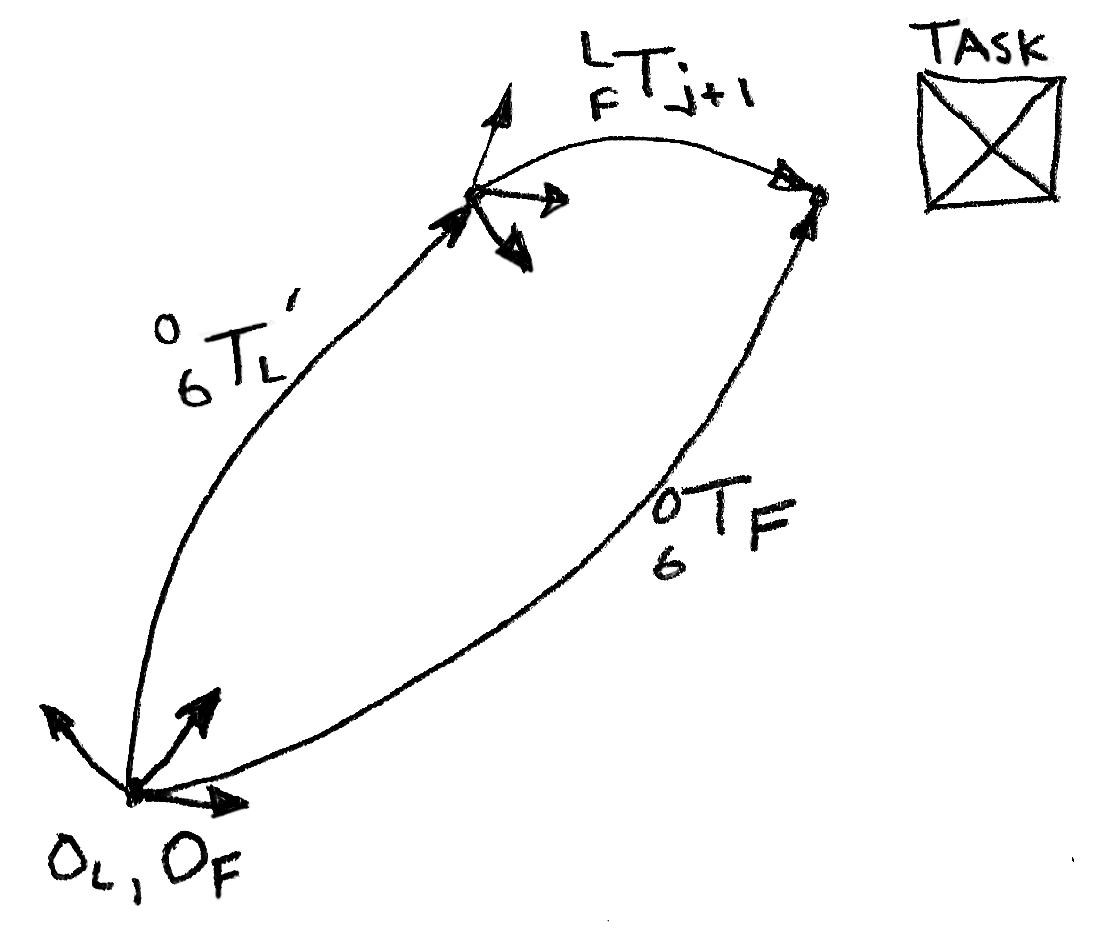
\includegraphics[width=3.0in]{figs14/00407a.png}

%\end{slide}
%\begin{slide}
%%%%** Section 2.5.2
\subsubsection{Procedure for Change of Index Offset}

\noindent
1) Normal Teleoperation:
\bq
^0_6T_F = ^0_6T_L(t)^L_FT_j
\eq

\noindent
2) Operator presses and holds index button:


\bq
\mathrm{Follower \quad position \quad locked} \qquad ^0_6T_F = constant
\eq

\noindent
3) Operator moves to new position, $^0_6T'_L$:

\bq
^L_FT_{j+1} = \left (^0_6T'_L\right )^{-1} {^0_6T_F}
\eq

\noindent
4) Resume Manipulation:

\bq
^0_6T_F = ^0_6T_L(t)^L_FT_{j+1}
\eq




%\end{slide}
%\begin{slide}

%%%%** Section 2.5.3
\subsubsection{Indexing (using incremental cartesian commands)}

Easier!


\bq\label{IncTeleop}
\Delta X_F = \Delta X_L = X_L(t) - X_L(t-\Delta t)
\eq

to index:
\begin{enumerate}
	\item Set $\Delta X_F = 0$
	\item Move leader device to new position.
	\item resume teleoperation using equation \ref{IncTeleop}
\end{enumerate}


%\end{slide}
%\begin{slide}
%%%%** Section 2.5.4
\subsubsection{Scaling (using 4x4 Frames)}

We might apply the following method to scale the command to the follower:
\bq
^0_6T_F =  \lambda_p I \left (
                 {^0_6T_L}{^L_FT_j}
                 \right )
\eq
this is {\bf not} OK.  (Why?)

However we could break inside the $T$ matrix and use

\bq
^0_6T_F = \left [
 \begin{array}{cc}
     \left [ R \right ]      & \lambda_p \left [ \begin{array}{c} P_x \\ P_y \\  P_z \end{array}\right ] \\
     \left [ 0 \quad 0 \quad 0 \right ] & 1 \\
 \end{array}
\right]
\eq

because orientation is not scaled by $\lambda_p$.


%\end{slide}
%\begin{slide}

%%%%** Section 2.5.5
\subsubsection{Scaling (using incremental cartesian commands)}


\bq
\Delta x_F = \lambda_p \Delta x_L
\eq

Simple!


%\end{slide}
%\begin{slide}


%%%%** Section 2.5.6
\subsubsection{Rate Control Option for Generalized Leader Follower}


Resolved rate control is an option which can be software selected in a generalized leader follower system.	%<hn>

\bq
\Delta x_F = \alpha_i(x_L-x_0)
\eq
where $x_0$ is a zero reference position such as the middle of the leader device motion range.	%<hn>

In this mode, the follower moves with a velocity proportional to the leader deflection
To make sure the follower velocity stays under control, there is a need
for a hardware or software spring return function to automatically set the leader
command to zero when there is no user force applied. 

%\end{slide}
%\begin{slide}

%%%%** Section 3
\section{Position Teloperation Kinematics: Summary}

Modes:

\begin{itemize}
	\item Joint Rate Control
	\item Resolved Rate Control
	\item Leader Follower Control
	\item Generalized Leader Follower Control
\end{itemize}

%\end{slide}
%\begin{slide}

\begin{tabular}{l|cccc}
                & Indexing         & Scaling        & Kinesthesia      & Ease   \\ \hline
Joint Rate      &    Y             &   Y            &    N             &  Low     \\
Resolved Rate   &    Y             &   Y            &    N             &        \\
Leader Follower    &    N             &   N            &    Y             &        \\
Generalized Leader Follower
                &    Y             &   Y            &    Y             & High  \\ \hline
\end{tabular}






\section{Applications}


\section{Summary of Notation}

% Summary of Notation for Chapter  14


